\begin{wrapfigure}{r}{0.25\textwidth}
\centering
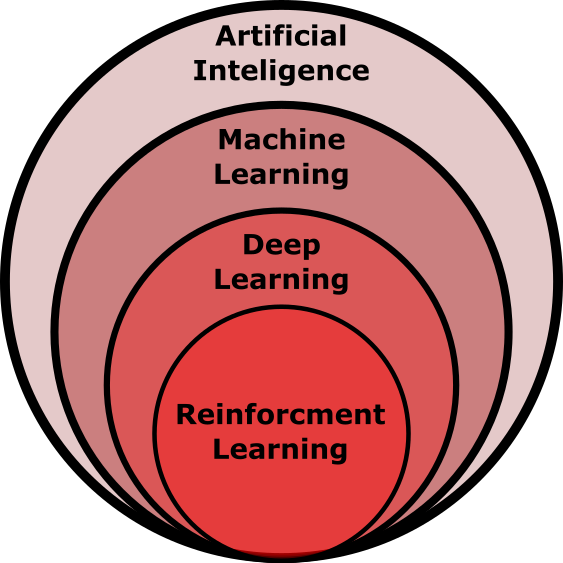
\includegraphics[width= 0.25\textwidth]{figures/AI Subsets.png}
\caption{Reinforcement learning subset}
\label{fig:sub}
\end{wrapfigure}

\section{Machine learning problem}
Machine learning is a subset of artificial intelligence, and deep learning is a subset of Machine learning. Deep learning classifies machine learning that uses deep neural networks. The neural network used in this scenario is an actor-critic, reinforcement learning (RL) approach
that reaches an optimal solution through the simulation of multiple episodes.\cite{rl2}

\subsection{Neural networks and deep learning}

  Artificial neural networks (ANN) are comprised of the input layer, hidden layers and the output layer. There can be many hidden layers constructed using perceptrons, the building block of an ANN, that map the inputs to the outputs. ANNs can have multiple inputs and outputs behaving as a MIMO controller and can map highly nonlinear input functions to any output signal. This is why they are commonly termed universal approximators.
\begin{figure}[h]
\centering
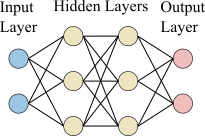
\includegraphics[width= 0.3\textwidth]{figures/NeuralNetwork.png}
\caption{Artificial Neural Network}
\label{fig:neu}
\end{figure}

\subsubsection{Perceptron}
The perceptron, shown in figure \ref{fig:per} is the activation function of a weighted sum.
\begin{figure}[h]
\centering
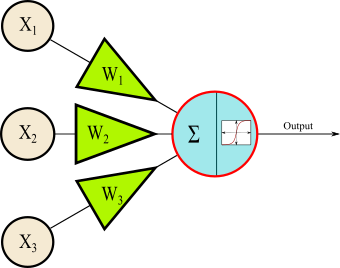
\includegraphics[width= 0.25\textwidth]{figures/Perceptron.png}
\caption{Perceptron}
\label{fig:per}
\end{figure}


\noindent
So with inputs and weight are:

\[\textbf{\textit{x}} = [x_1,x_2,...,x_k] , \textbf{\textit{w}} = [w_1,w_2,...,w_k]\]

\noindent
then, 

\[\textbf{\textit{x}} \cdot \textbf{\textit{w}} + b = 0\]
\noindent
The hidden layers made up of perceptrons change their weights and biases through back-propagation in the direction suggested by the loss function covered later on. In this case, the actor-critic network is used.

\clearpage
\subsubsection{Activation function}
An activation function is used since this allows the agent to map complex relationships of output and input. It can vary but, in this case, the sigmoid function is used as it can map continuous functions from \(0\) to \(1\).

\begin{equation}\centering
\vcenter{\hbox{\begin{minipage}{7cm}
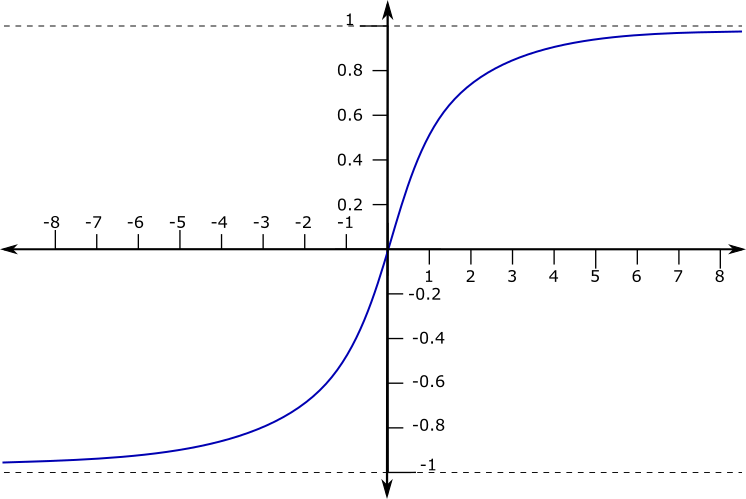
\includegraphics[width=5cm]{figures/Sigmoid.png}
\captionof{figure}{Sigmoid activation Function}
\end{minipage}}}
\qquad\qquad
\begin{aligned}
\sigma(z) = {1\over{1+e^{-z}}}
\end{aligned}
\end{equation}

As the input goes from \(-\infty\) to \(+\infty\) the output ranges from \(0\) to \(1\). This means large differences in the input are normalised which allows the network to learn highly non-linear functions.
\clearpage
\subsection{Reinforcement Learning}
\begin{wrapfigure}{r}{0.4\textwidth}
  \begin{center}
    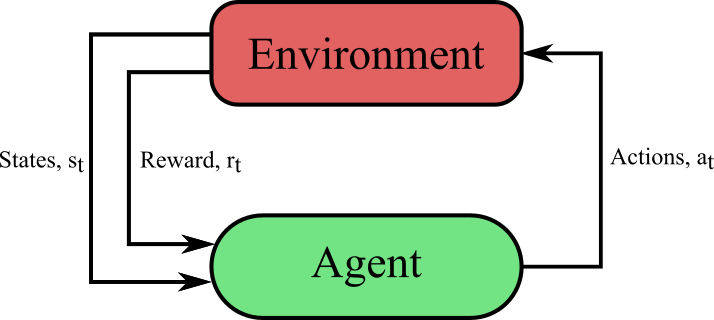
\includegraphics[width=0.4\textwidth]{figures/EnvironmentAgent.png}
    \end{center}
    \caption{Reinforcement learning Agent}
    \label{fig:Actor agent}
\end{wrapfigure}

Reinforcement learning (RL) \cite{rl1} is used to optimise complex or unpredictable control. The agent interacts with an environment to maximise reward. At each discrete time step $t$, with a given state $s \in S$ the agent chooses an action $a_t \in A$ with respect to the policy function $\pi : S \xrightarrow{} A$. The agent then receives a reward $r_{t+1}$ and a new state $s_{t+1}$ for that action\cite{ac1}. This model is known as a Markov Decision Process(MPD)\cite{mar1}, which means the agent acts in a discrete, stochastic, sequential environment.

\subsubsection{Policy}
Policy \begin{math}\pi_\theta(s_t,a_t)\end{math} can be either Stochastic or deterministic:

\begin{itemize}
\item
\textbf{Deterministic} -
A policy is deterministic if there is a clear action for any state. This will not explore new options and is referred to as greedy. This would be a pre-trained agent which has a consistent behaviour.

\item
\textbf{Stochastic } -
This policy means that there is some statistical element of variation is included.  $ \pi_\theta(s_t,a_t) $ represents the conditional probability density at $a_t$ associated with the policy.\cite{ac2} 

\end{itemize}

In this case, the policy \begin{math}\pi_\theta(s_t,a_t)\end{math} behaves stochastically with the MPD environment such that:

 \[s_0,a_0,r_1,s_1,a_1,r_2, ... ,s_{k-1},a_{k-1},r_n,s_k\]

The policy $\pi_\theta(s_t,a_t)$ is a neural network with policy parameters $\theta$ which are initialised at arbitrary values. The policy parameter are then changed using the policy gradient theorem covered later\cite{rl2} to maximise long cumulative reward.
 
\subsubsection{Reward}

The return at time step t is is defined as the discounted sum of rewards:

\[r_t^\gamma =  r_t + \gamma r_{t+1} +\gamma^2 r_{t+2} + ... +\gamma^{k-t} r_k\]

\noindent

Return is often expressed as $G_t$ and can be represented as:

\begin{equation}
     G_t = r_t^\gamma = \sum_{k =  t}^T\gamma^{k-t}r(s_k,a_k)
     \label{equ:rew}
\end{equation}

Where discount factor $0< \gamma < 1$  determines the priority of the short term rewards. This  pushes the agent to finish the simulation faster as it decreases since the short term reward is less valuable than long term reward.

\subsubsection{Value function and bellman optimality}
A value function is defined as the estimated total discounted reward. In this case, a Q-actor-critic network is used which means the \textbf{state-action} value function \cite{ac2} is used:


\[Q^{\pi}(s_t,a_t) = \mathbb{E}[G_t | s_t = s, a_t = a;\pi]\]


This equation provides a function that estimates the future reward with a given initial state following the current policy. Since this is a maximisation problem the optimal state-value \cite{bel1} the optimal state-action value function indicates the maximum reward:

\[Q_*(s,a) = \mathop{max}_{\pi}Q_\pi(s,a)\]

\noindent
\textbf{Bellman Optimality Equation}\\


Bellman proved that optimal action value function $Q_*$ satisfies:

\begin{equation}
Q_*(s,a) = \mathbb{E}[r_{t+1} + \gamma\mathop{max}_{a'}Q_*(s',a')]
\label{equ:bel}
\end{equation}

This means that at time $t$, for any state-action pair $(s,a)$, the expected return from a given state $s$ and action $a$, using the optimal policy function will be the sum of the expected reward $r_{t+1}$ achieved through action $a$ and the maximum expected discounted reward, achievable for any $(s',a')$. $(s',a')$ are the expected next state-action pair. $s'$ will be the state from which the best action $a'$ can be taken at time $t+1$.\cite{bel2}\hfill
\newline
\newline
\noindent
\textbf{Loss function}\\

To converge to an optimal solution the agent then acts to find the actual $Q(s,a)$. The loss is defined as the difference between the optimal Q-value and the optimal Q-value so the loss is $Q_*(s,a)-Q(s,a)$. They are compared iteratively until the value function converges to the optimal solution:

\begin{equation}
    Q'(s,a) = (1-\alpha)\underbrace{Q(s,a)}_\text{Old value} + \alpha\overbrace{[r_{t+1} + \gamma\mathop{max}_{a'}Q_*(s',a')}^\text{Learned value} ]
\end{equation}
Where $\alpha$ is the learning rate which determines how much of the information the previously computed Q-value will remain in the next iteration.


\clearpage
\subsubsection{Policy Gradient theorem}\label{GOAL}
The reinforcement learning objective is to maximise long term cumulative reward. this can be formulated as:

\begin{equation}
    J(\theta) = \mathbb{E}[\sum_{t=0}^{T-1} r_{t+1}]
    \label{equ:re}
\end{equation}

In every iteration, the policy parameter is changed through back-propagation in the direction of gradient ascent as this is a maximisation problem:

\[\theta \xleftarrow{} \theta + {\partial\over{\partial\theta}}J(\theta)\]


\noindent
Derived in \cite{neu2}, the policy gradient is then.

\begin{equation}
    \nabla_\theta J(\theta) = \mathbb{E}[\sum_{t=0}^{T-1} \nabla_\theta log\pi_\theta (a_t|s_t)Q(s,a)]
    \label{equ:grad}
\end{equation}

\noindent
The reinforce algorithm is a Monte-Carlo\cite{mon1} variant of policy gradients. This is a statistical method that chooses random samples so that agents can explore different policies.





\subsubsection{Actor-Critic Methods}
The overall aim of this optimization function is to reduce the loss function through back-propagation and gradient ascent\cite{ac1}.The Q-actor-critic achieves this with 2 parametrised neural networks:

\begin{itemize}
    \item 
    \textbf{Value critic} -
    estimates the state-action value from Bellman equation \ref{equ:bel}.
    \item 
    \textbf{Policy actor} -
    This updates the policy in the direction suggested by the critic through gradient ascent in equation \ref{equ:grad}.
\end{itemize}


\clearpage